\documentclass[10pt]{article}

% File icdp2009.sty
% Preamble that you have to include to use the template  

% July 24, 2009
% Contact: simonnet@ecole.ensicaen.fr


\usepackage[a4paper,textwidth=18cm,textheight=24cm,top=2.85cm, bottom=2.85cm, left=1.5cm, right=1.5cm]{geometry}

\usepackage{../template/icdp2009}

% left justified caption
\makeatletter
\long\def\@makecaption#1#2{%
\vskip\abovecaptionskip
\sbox\@tempboxa{#1. #2}%
\ifdim \wd\@tempboxa >\hsize
#1. #2\par
\else
\global \@minipagefalse
\hb@xt@\hsize{\box\@tempboxa\hfil}%
\fi
\vskip\belowcaptionskip}
\makeatother




%other package

% vectorial font
\usepackage{lmodern}

\usepackage{graphicx}
\usepackage{times}
\usepackage{booktabs}
\usepackage{siunitx}
\usepackage{adjustbox}
\usepackage{multirow}


\begin{document}
\noindent

% This should produce references in the order they appear
\bibliographystyle{ieeetr}

\title{Optical Waveguides: Theory and Implementation}

\authorname{Anirudh Prakash, Grace Liu, Surya Chandramouleeswaran}
\authoraddr{\textbf{\emph{A special thanks to Professor Maysam Chamanzar}}}



\maketitle


\abstract
Replace this with a succint summary of our work. Aim for 100 words  

\section{Introductory Concepts and Motivations}

Discuss introductory concepts here, something like motivations works well too


\begin{figure}[h]
    \centering
    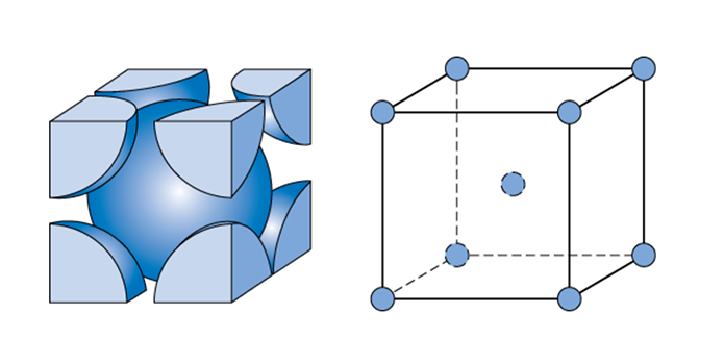
\includegraphics[width=8.5cm]{fig1.eps}
    \caption{\label{tab1}BCC Unit Cell structure, with an atom at the center of the "body" of the cell. Adapted from \cite{ref01}.} 
    \end{figure}

\section{Historical Contextualizations}

Include timeline diagrams and discuss some important context details here.


\begin{figure}[h]
    \centering
    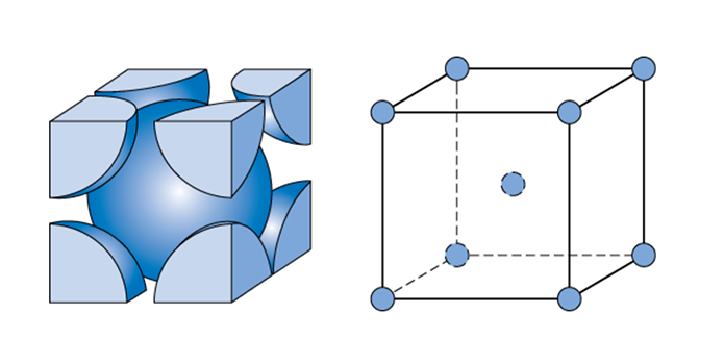
\includegraphics[width=8.5cm]{fig1.eps}
    \caption{\label{tab1}BCC Unit Cell structure, with an atom at the center of the "body" of the cell. Adapted from \cite{ref01}.} 
    \end{figure}

\section{Propagation of Light}

Here we discuss EM mechanisms. Start fundamental and work our way up 


\begin{figure}[h]
    \centering
    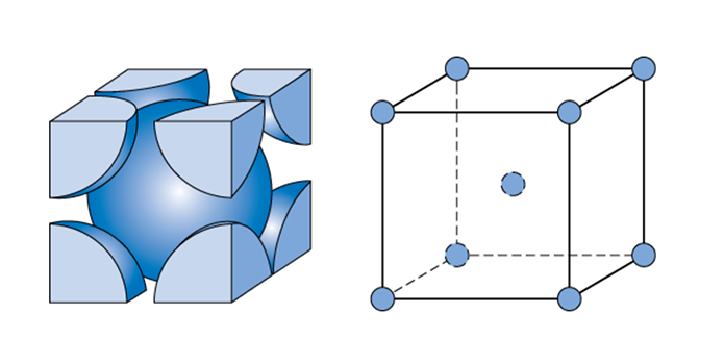
\includegraphics[width=8.5cm]{fig1.eps}
    \caption{\label{tab1}BCC Unit Cell structure, with an atom at the center of the "body" of the cell. Adapted from \cite{ref01}.} 
    \end{figure}

\section{Electromagnetic Mechanisms}

More speciffc here, add TIR and add diagrams and math

\begin{figure}[h]
    \centering
    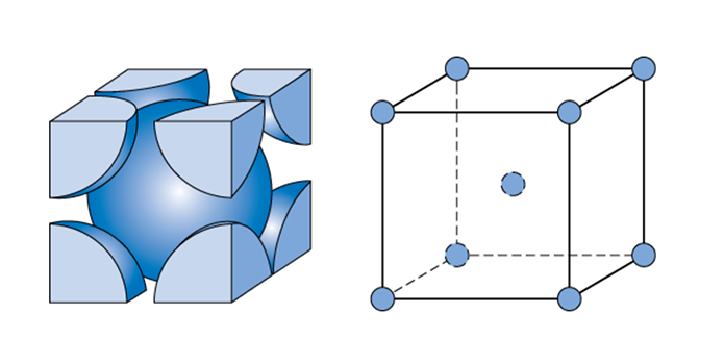
\includegraphics[width=8.5cm]{fig1.eps}
    \caption{\label{tab1}BCC Unit Cell structure, with an atom at the center of the "body" of the cell. Adapted from \cite{ref01}.} 
    \end{figure}

\section{System Integration}

Transitions into some more implmentation details that bleeds into state of art discussion 


\begin{figure}[h]
    \centering
    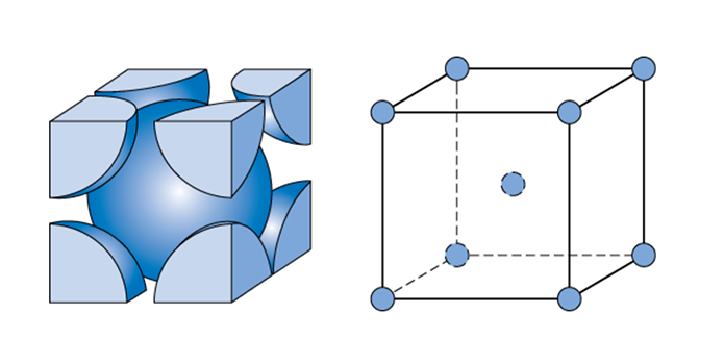
\includegraphics[width=8.5cm]{fig1.eps}
    \caption{\label{tab1}BCC Unit Cell structure, with an atom at the center of the "body" of the cell. Adapted from \cite{ref01}.} 
    \end{figure}

\textbf{Anirudh}: you can decide how you want to organize this 

\section{Evaluation of the State of the Art}

PIC discussion, materials perspective, etc.



\section{Concluding Thoughts and Ideas for the Future}

self explanatory 




\section{Acknowledgements}

bibliography is very important (references section needs to be modified in example.bib)
\bibliography{IEEEabrv,icdp2009}


\end{document}














